% tikz_stop.tex -- why the pair terms cannot settle twenty-four centres (Section 2.8).
%   (a) The section of the 24-cell Q = {x : <x, y> <= |y|^2/2 for the 24 centres y of
%       sqrt2 R} by the plane x3 = x4 = 0: the square |x1| + |x2| <= sqrt2, whose sides
%       touch the unit ball (radius 1) and whose corners are vertices of Q at radius
%       sqrt2.  The ball of radius sqrt(3/2), inside which Lemma 2.15 makes the cell an
%       exact function of the pairs, cuts the four corners off (orange).  In R^4 the 24
%       such corners hold 8 - 7.906940 = 0.093060 of the volume.  The four centres of
%       the plane, sqrt2(+-e1 +- e2), at distance 2, and their inversion hull (dashed
%       square) through the corners.  To scale.
%   (b) One corner, magnified: the vertex v = sqrt2 e1, the two sides through it, the
%       arc of radius sqrt(3/2), the side x1 = sqrt2 of the hull, which touches Q only
%       at v, and the depth sqrt2 - sqrt(3/2) = 0.189 of the corner.  To scale.
% Build:  pdflatex tikz_stop.tex && pdftoppm -r 500 -png -singlefile tikz_stop.pdf ../figures/fig_tikz_stop
\documentclass[border=4pt]{standalone}
\usepackage{tikz}
\usetikzlibrary{calc,arrows.meta}
\usepackage[T1]{fontenc}
\usepackage{lmodern}
\usepackage{amsmath,amssymb}
\definecolor{cblue}{HTML}{2A78D6}
\definecolor{corange}{HTML}{EB6834}
\definecolor{caqua}{HTML}{1BAF7A}
\definecolor{cviolet}{HTML}{4A3AA7}
\definecolor{cink}{HTML}{0B0B0B}
\definecolor{cink2}{HTML}{52514E}
\definecolor{cink3}{HTML}{8B8A85}
\begin{document}
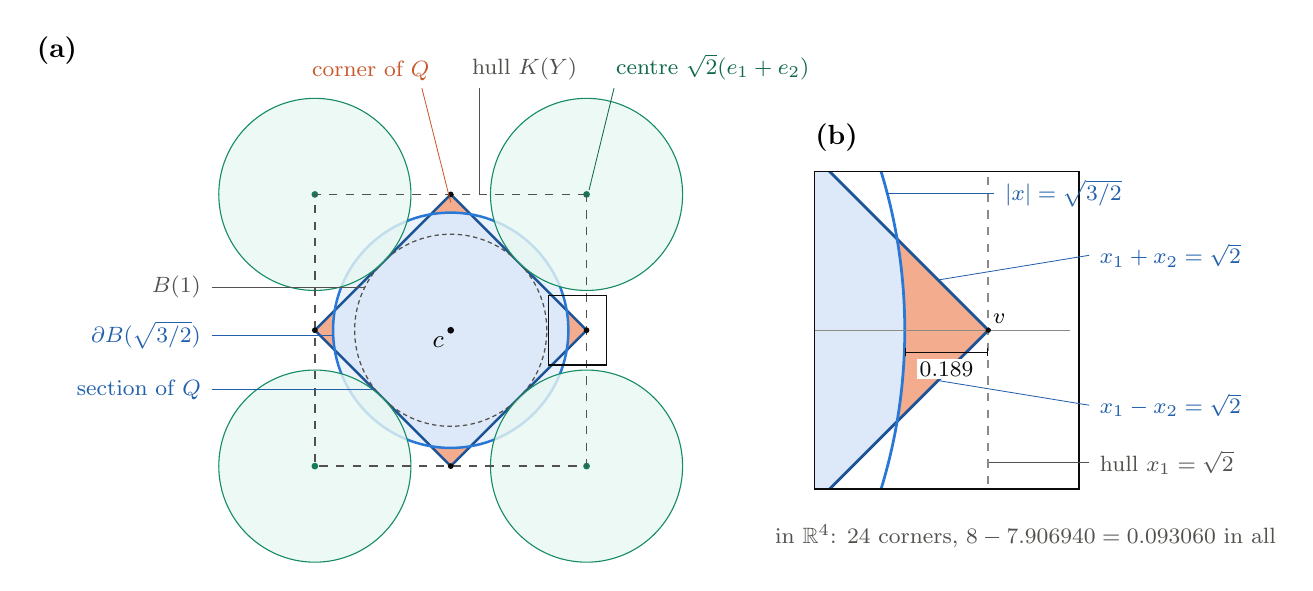
\begin{tikzpicture}[font=\small]
\pgfmathsetmacro{\sq}{sqrt(2)}
\pgfmathsetmacro{\R}{sqrt(1.5)}
\pgfmathsetmacro{\cx}{sqrt(1.5-0.5*0)}        % unused helper
%% ------------------------------------------------------------------ (a)
\begin{scope}[scale=1.22]
  % the corners of Q beyond the ball of radius sqrt(3/2): Q minus the disc
  \begin{scope}
    \clip (\sq,0) -- (0,\sq) -- (-\sq,0) -- (0,-\sq) -- cycle;
    \fill[corange!55, even odd rule] (-2,-2) rectangle (2,2) (0,0) circle (\R);
  \end{scope}
  % the section of Q, the square |x1| + |x2| <= sqrt2
  \fill[cblue!10] (0,0) circle (\R);
  \begin{scope}
    \clip (0,0) circle (\R);
    \fill[cblue!16] (\sq,0) -- (0,\sq) -- (-\sq,0) -- (0,-\sq) -- cycle;
  \end{scope}
  \draw[cblue!70!black, line width=0.9pt] (\sq,0) -- (0,\sq) -- (-\sq,0) -- (0,-\sq) -- cycle;
  % the unit ball and the ball of radius sqrt(3/2)
  \draw[cink2, line width=0.45pt, dash pattern=on 1.6pt off 1.2pt] (0,0) circle (1);
  \draw[cblue, line width=0.9pt] (0,0) circle (\R);
  % the four centres, at distance 2, and their unit balls, which touch the unit ball
  \foreach \a in {45,135,225,315} {
    \draw[caqua!80!black, line width=0.4pt, fill=caqua!10, fill opacity=0.8] (\a:2) circle (1);
    \fill[caqua!70!black] (\a:2) circle (0.035);
  }
  \draw[cink2, dashed, line width=0.55pt] (\sq,\sq) -- (-\sq,\sq) -- (-\sq,-\sq) -- (\sq,-\sq) -- cycle;
  \fill[cink] (0,0) circle (0.035);
  \node[below left=-1pt] at (0,0) {$c$};
  % the vertices of Q in the plane
  \foreach \p in {(\sq,0),(0,\sq),(-\sq,0),(0,-\sq)} \fill[cink] \p circle (0.03);
  % labels, each on a leader line to a free spot
  \node[caqua!60!black, anchor=south west, font=\footnotesize] at (1.62,2.5) {centre $\sqrt2(e_1+e_2)$};
  \draw[caqua!60!black, line width=0.3pt] (1.7,2.52) -- (1.44,1.46);
  \node[cink2, anchor=south west, font=\footnotesize] at (0.12,2.5) {hull $K(Y)$};
  \draw[cink2, line width=0.3pt] (0.3,2.52) -- (0.3,1.414);
  \node[corange!85!black, anchor=south east, font=\footnotesize] at (-0.12,2.5) {corner of $Q$};
  \draw[corange!85!black, line width=0.3pt] (-0.3,2.52) -- (0,1.33);
  \node[cink2, anchor=east, font=\footnotesize] at (-2.5,0.45) {$B(1)$};
  \draw[cink2, line width=0.3pt] (-2.49,0.45) -- (-0.893,0.45);
  \node[cblue!80!black, anchor=east, font=\footnotesize] at (-2.5,-0.05) {$\partial B(\sqrt{3/2})$};
  \draw[cblue!80!black, line width=0.3pt] (-2.49,-0.05) -- ({-sqrt(1.5-0.0025)},-0.05);
  \node[cblue!80!black, anchor=east, font=\footnotesize] at (-2.5,-0.62) {section of $Q$};
  \draw[cblue!80!black, line width=0.3pt] (-2.49,-0.62) -- (-0.794,-0.62);
  % the frame of panel (b)
  \draw[cink, line width=0.5pt] (1.02,-0.36) rectangle (1.62,0.36);
\end{scope}
\node[font=\bfseries] at (-5.0,3.55) {(a)};
%% ------------------------------------------------------------------ (b)
\begin{scope}[xshift=6.3cm, scale=5.6, shift={(-1.32,0)}]
  \begin{scope}
    \clip (1.02,-0.36) rectangle (1.62,0.36);
    % inside the ball: the cell, pale
    \begin{scope}
      \clip (\sq,0) -- (0,\sq) -- (-\sq,0) -- (0,-\sq) -- cycle;
      \fill[cblue!16] (0,0) circle (\R);
      \fill[corange!55, even odd rule] (0.9,-0.6) rectangle (1.7,0.6) (0,0) circle (\R);
    \end{scope}
    \draw[cblue!70!black, line width=1.0pt] (\sq,0) -- (0,\sq);
    \draw[cblue!70!black, line width=1.0pt] (\sq,0) -- (0,-\sq);
    \draw[cblue, line width=1.0pt] (0,0) circle (\R);
    \draw[cink3, dashed, line width=0.6pt] (\sq,-0.5) -- (\sq,0.5);
    \draw[cink2, line width=0.45pt, dash pattern=on 1.6pt off 1.2pt] (0,0) circle (1);
    % the direction of the vertex, from c
    \draw[cink3, line width=0.35pt] (0.9,0) -- (1.6,0);
  \end{scope}
  \draw[cink, line width=0.5pt] (1.02,-0.36) rectangle (1.62,0.36);
  \fill[cink] (\sq,0) circle (0.006);
  % the depth of the corner
  \draw[{Bar[width=3pt]}-{Bar[width=3pt]}, cink, line width=0.5pt] (\R,-0.05) -- (\sq,-0.05);
  \node[below=1pt, cink, font=\footnotesize, fill=white, inner sep=1pt] at ({(\R+\sq)/2},-0.058) {$0.189$};
  \node[anchor=south west, font=\footnotesize, inner sep=1.5pt] at (\sq,0.004) {$v$};
  \node[cblue!80!black, font=\footnotesize, anchor=west] at (1.43,0.31) {$|x|=\sqrt{3/2}$};
  \draw[cblue!80!black, line width=0.3pt] (1.428,0.31) -- ({sqrt(1.5-0.31*0.31)},0.31);
  \node[cink2, font=\footnotesize, anchor=west] at (1.645,-0.3) {hull $x_1=\sqrt2$};
  \draw[cink2, line width=0.3pt] (1.643,-0.3) -- (1.416,-0.3);
  \node[cblue!80!black, font=\footnotesize, anchor=west] at (1.645,0.17) {$x_1+x_2=\sqrt2$};
  \draw[cblue!80!black, line width=0.3pt] (1.643,0.17) -- (1.30,0.114);
  \node[cblue!80!black, font=\footnotesize, anchor=west] at (1.645,-0.17) {$x_1-x_2=\sqrt2$};
  \draw[cblue!80!black, line width=0.3pt] (1.643,-0.17) -- (1.30,-0.114);
\end{scope}
\node[font=\bfseries] at (4.9,2.45) {(b)};
\node[font=\footnotesize, cink2, align=center, anchor=north] at (7.3,-2.35)
  {in $\mathbb{R}^4$: $24$ corners, $8-7.906940=0.093060$ in all};
\end{tikzpicture}
\end{document}
